\chapter{Technical Issues}

\section{NJTREE Software}

NJTREE is the core engine of the whole TreeFam database. It realizes
almost all the algorithms described in this thesis, including
the cNJ algorithm (Section~\ref{sec:cnj}) for both rooted and unrooted constraining trees,
rooting and bootstrapping,
leaf reording algorithm (Section~\ref{sec:reorder}),
duplication/loss inference for multifurcated species trees (Chapter~\ref{chap:dli}),
and tree merge algorithm (Chapter~\ref{chap:merge}.
It also provides a lot of utilities facilitating the construction of TreeFam (Chapter~\ref{chap:treefam})
and the benchmark done in Chapter~\ref{chap:benchmark}.
In addition, NJTREE incorporates source codes from PHYML~\cite{guindon03},
which makes it capable of utilizing the power of ML methods.
To some extent, most parts of the thesis is describing the priciples behind this software.

NJTREE is efficient. It is much faster than any other neighbour-joining tree builders,
and can calculate max-likelihood distance in a speed not compared by other
similar softwares. Even NJTREE-revised PHYML codes runs 20\% faster than the original ones.
In addition, NJTREE comes with a nice graphical user interface (GUI), FLNJTREE, which is built upon
FLTK (fast light-weighted toolkit), a cross-platform widget library. FLNJTREE
can be compiled in both UNIX (including LINUX) and Windows. In theory, it should also work in Mac OSX, though this
has not been tested. Figure~\ref{fig:flnjtree} shows a snapshot of FLNJTREE.

\begin{figure}[!hb]
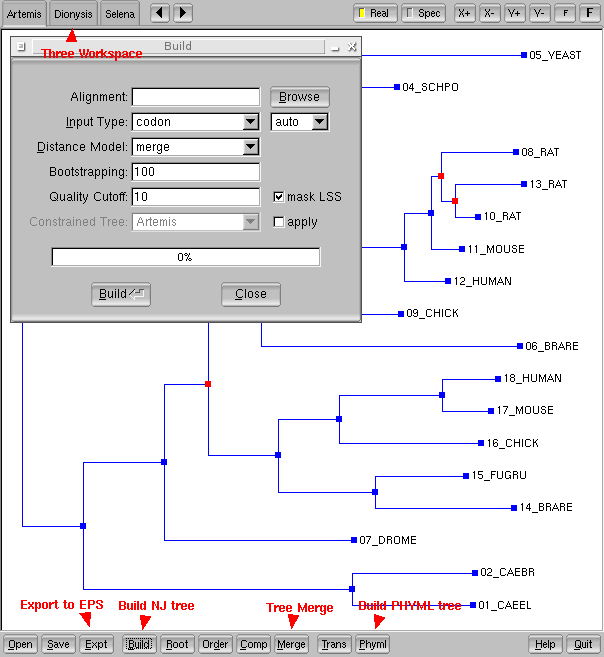
\includegraphics[width=\textwidth]{flnjtree.png}
\caption{Screenshot of FLNJTREE software.}\label{fig:flnjtree}
\end{figure}

\section{MySQL Structures}
TreeFam database is supported on \href{http://www.mysql.com/}{MySQL}, probably
the most popular open source database in the world. Except the original
PhIGs alignment, all the other data are stored in the relational database.
The structures of TreeFam MySQL schema are very intuitive.
Most the tables can be classified into three groups: tables for describing
gene attributes, tables for recording family information, and tables connecting
the two parts. Table~\ref{tab:mysql-table} gives a brief list of key tables
in TreeFam database, and Figure~\ref{fig:schemata} shows the relations between them.
Note that in TreeFam MySQL tables, gene identifiers and family accessions are
directly used as index. This is clearer than using integer ID, but is ineffiecient from
a pure technical angle~\footnote{\href{http://www.informit.com/articles/article.asp?p=377652\&seqNum=1}
{http://www.informit.com/articles/article.asp?p=377652\&seqNum=1}}. As efficiency seems not a serious problem at present,
we can live with this for the moment. TreeFam MySQL database is open to public at
{\bf db.treefam.org:3308}. The read-only account is {\bf anonymous} with empty password.

\begin{figure}[!hb]
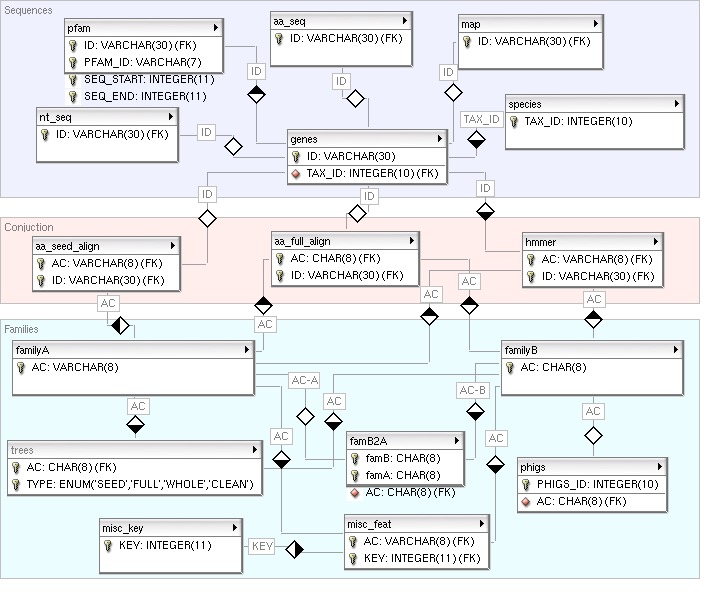
\includegraphics[width=\textwidth]{schemata.png}
\caption[Schema of TreeFam database]{Schema of TreeFam database. This figure is generated by
\href{http://www.fabforce.net/dbdesigner4/}{DBDesigner4}.}\label{fig:schemata}
\end{figure}

\begin{table}[!hb]
\begin{center}
\begin{tabular}{|l|l|}
\hline
Table & Description \\
\hline
genes & sequence ID, gene name, transcript name, symbol, description and so on \\
species & tax ID, taxonomy name, {\it abbr.} name, and common name of species \\
map & genomic locations of transcripts; in UCSC format \\
pfam & Pfam predictions for each sequence \\
aa\_seq & amino acid sequences \\
nt\_seq & nucleotide sequences \\
familyA & accessions, symbols and names of TreeFam-A families \\
familyB & basic information on TreeFam-B families \\
famB2A & relation between curated TreeFam-A and original TreeFam-B families \\
phigs & PhIGs accessions of TreeFam-B families \\
trees & phylogenetic trees in NHX format \\
misc\_feat & symbols and names of B families; curators of A families \\
misc\_key & descriptions of `key' used in `misc\_feat' table \\
aa\_seed\_align & amino acids multialignment for TreeFam-A seeds in CIGAR format \\
aa\_full\_align & full multialignment for both A and B families in CIGAR format \\
hmmer & HMMer scores of matched sequences \\
\hline
\end{tabular}
\end{center}
\caption[Description of key TreeFam MySQL tables]{Description of key TreeFam MySQL tables. Trivial or obsolete ones
are not included.}\label{tab:mysql-table}
\end{table}

\section{Perl API}
It is recommended to connect TreeFam MySQL with perl API, which
provides convenient interface for the retrieval of various TreeFam data. TreeFam API
also implements a light-weighted parser for NHX format, a versatile tree plotter and
a simple alignment plotter. Full documentation is available at
\href{http://www.treefam.org/api/}{http://www.treefam.org/api/}.
%We only show some practical examples here as an introduction.
